\documentclass[11pt,a4paper]{article}

% ---------------------------------------------------------------
% Pacotes
% ---------------------------------------------------------------
\usepackage[T1]{fontenc}
\usepackage[utf8]{inputenc}
\usepackage[brazil]{babel}
\usepackage{lmodern}
\usepackage{microtype}
\usepackage[margin=2.5cm]{geometry}
\usepackage{amsmath}
\usepackage{booktabs}
\usepackage{tabularx}
\usepackage{graphicx}
\usepackage{float}
\usepackage[font=small,labelfont=bf]{caption}
\usepackage{xcolor}
\usepackage[hidelinks]{hyperref}

\definecolor{verde}{HTML}{1F3B2D}
\newcolumntype{R}{>{\raggedleft\arraybackslash}p{1.7cm}}

% Números gerados pelo script gerar_resultados.py
\newcommand{\NumLinhas}{38.765}
\newcommand{\NumProdutos}{167}
\newcommand{\NumClientes}{3.898}
\newcommand{\NumCompras}{14.963}
\newcommand{\NumComprasRUm}{14.963}
\newcommand{\MediaItens}{2,6}
\newcommand{\MediaItensUnicos}{2,5}
\newcommand{\NumUmItemUnico}{205}
\newcommand{\NumFrequentesRUm}{750}
\newcommand{\NumRegrasRUm}{240}
\newcommand{\NumRegrasUnicasRUm}{120}
\newcommand{\MaxConfRUm}{25,6}
\newcommand{\PctConfVinte}{99}
\newcommand{\PctSupBaixo}{85}
\newcommand{\CorrLiftConf}{0,12}
\newcommand{\MelhorLift}{2,18}
\newcommand{\MelhorConf}{13,2}
\newcommand{\MelhorCompras}{22}
\newcommand{\MinComprasRUm}{15}
\newcommand{\NumComprasRDois}{12.270}
\newcommand{\NumFrequentesRDois}{1.260}
\newcommand{\NumRegrasRDois}{432}
\newcommand{\NumRegrasUnicasRDois}{216}
\newcommand{\MinComprasRDois}{6}
\newcommand{\SigRUm}{7}
\newcommand{\SigRDois}{10}
\newcommand{\BonfRUm}{0}
\newcommand{\BonfRDois}{0}
\newcommand{\BonfTodasRUm}{0}
\newcommand{\BonfTodasRDois}{0}
\newcommand{\AlfaBonfRUm}{0,00042}
\newcommand{\AlfaBonfRDois}{0,00023}
\newcommand{\MenorPRUm}{0,00045}
\newcommand{\MenorPRDois}{0,0029}
\newcommand{\BHRUm}{0}
\newcommand{\BHRDois}{0}
\newcommand{\MenorQRUm}{0,054}
\newcommand{\MenorQRDois}{0,43}
\newcommand{\TopUmPct}{15,8}


% ---------------------------------------------------------------
\title{\textbf{Mineração de Regras de Associação\\no Groceries Dataset}\\[6pt]
\large O que os clientes compram juntos?}
\author{Ailana \qquad André \qquad Pedro \qquad Victor\\[8pt]
\normalsize Inteligência Computacional --- Prof.\ Canarozzo}
\date{25 de novembro de 2026}

\begin{document}

\maketitle

\begin{abstract}
Este trabalho aplica o algoritmo Apriori a \NumLinhas{} registros de compras de supermercado, agrupados em \NumCompras{} transações, para encontrar produtos que costumam ser comprados juntos. Com suporte mínimo de 0,1\%, foram encontrados \NumFrequentesRUm{} conjuntos frequentes e \NumRegrasUnicasRUm{} regras distintas com lift maior ou igual a 1. A regra mais forte, \emph{iogurte + leite integral $\rightarrow$ salsicha}, tem lift de \MelhorLift{}, mas aparece em apenas \MelhorCompras{} compras. Removendo os itens dominantes, surgem pares típicos de receitas, como presunto e conservas (lift 3,32). Um teste exato de Fisher indica que a maioria das regras do topo é significativa isoladamente; porém, após a correção para comparações múltiplas, nenhuma se sustenta. Concluímos que as regras descrevem tendências plausíveis, que devem ser confirmadas com mais dados antes de orientar decisões.
\end{abstract}

% ---------------------------------------------------------------
\section{Introdução}

Supermercados registram cada compra como uma lista de itens. Analisando milhares dessas listas, é possível descobrir quais produtos tendem a sair juntos no caixa. Essa técnica, chamada de \emph{análise de cesta de compras} (\emph{market basket analysis}), apoia decisões como a disposição dos produtos nas prateleiras, a criação de combos e promoções e os sistemas de recomendação do tipo ``quem comprou isto também comprou aquilo''.

O objetivo deste trabalho é aplicar a mineração de regras de associação a uma base pública de compras, interpretar as regras encontradas e avaliar o quanto elas são confiáveis. O código está no notebook \texttt{Mineração\_produtos.ipynb}, e todas as tabelas e figuras deste relatório são geradas pelo script \texttt{relatorio/gerar\_resultados.py}.

% ---------------------------------------------------------------
\section{Fundamentação teórica}

\subsection{Regras de associação}

Seja $I$ o conjunto de produtos e $T$ uma base de $N$ transações, cada uma um subconjunto de $I$. Uma \emph{regra de associação} é uma implicação $A \rightarrow B$, em que $A$ (antecedente) e $B$ (consequente) são conjuntos de produtos disjuntos~\cite{agrawal1993}. A regra é avaliada por três métricas:

\begin{align}
\text{suporte}(A \rightarrow B)   &= P(A \cap B) = \frac{|\{t \in T : A \cup B \subseteq t\}|}{N}, \\[4pt]
\text{confiança}(A \rightarrow B) &= P(B \mid A) = \frac{\text{suporte}(A \cup B)}{\text{suporte}(A)}, \\[4pt]
\text{lift}(A \rightarrow B)      &= \frac{\text{confiança}(A \rightarrow B)}{\text{suporte}(B)} = \frac{P(A \cap B)}{P(A)\,P(B)}.
\end{align}

O suporte mede o quanto o padrão é comum; a confiança, o quanto $A$ prevê $B$; e o lift compara a ocorrência conjunta com o que se esperaria se os produtos fossem independentes~\cite{brin1997}. Lift maior que 1 indica associação positiva, igual a 1 indica independência e menor que 1 indica que um produto tende a afastar o outro. Como o lift é simétrico, as regras $A \rightarrow B$ e $B \rightarrow A$ têm sempre o mesmo valor.

\subsection{O algoritmo Apriori}

O Apriori~\cite{agrawal1994} encontra todos os conjuntos de itens com suporte acima de um mínimo. Ele se baseia na propriedade de \emph{antimonotonicidade}: se um conjunto é frequente, todos os seus subconjuntos também são. Assim, o algoritmo gera candidatos de tamanho $k+1$ apenas a partir de conjuntos frequentes de tamanho $k$, descartando cedo grande parte das combinações possíveis. As regras são então derivadas dos conjuntos frequentes.

% ---------------------------------------------------------------
\section{Base de dados}

Foi usado o \emph{Groceries Dataset}~\cite{groceries}, em que cada linha registra um produto comprado por um cliente em uma data. Cada combinação de cliente e data foi tratada como uma transação. A Tabela~\ref{tab:dataset} resume a base.

\begin{table}[H]
\centering
\caption{Resumo do Groceries Dataset.}
\label{tab:dataset}
\begin{tabular}{lr}
\toprule
Informação & Valor \\
\midrule
Registros (linhas do CSV) & \NumLinhas \\
Transações (cliente + data) & \NumCompras \\
Clientes & \NumClientes \\
Produtos diferentes & \NumProdutos \\
Itens por transação (média) & \MediaItens \\
Itens distintos por transação (média) & \MediaItensUnicos \\
Período & 2014 e 2015 \\
\bottomrule
\end{tabular}
\end{table}

A distribuição dos produtos é bastante desigual. A Figura~\ref{fig:itens} mostra que o leite integral está em \TopUmPct\% das transações, seguido por outros vegetais, pãezinhos e refrigerante. Esses itens tendem a aparecer em muitas regras apenas por serem comuns.

\begin{figure}[H]
\centering
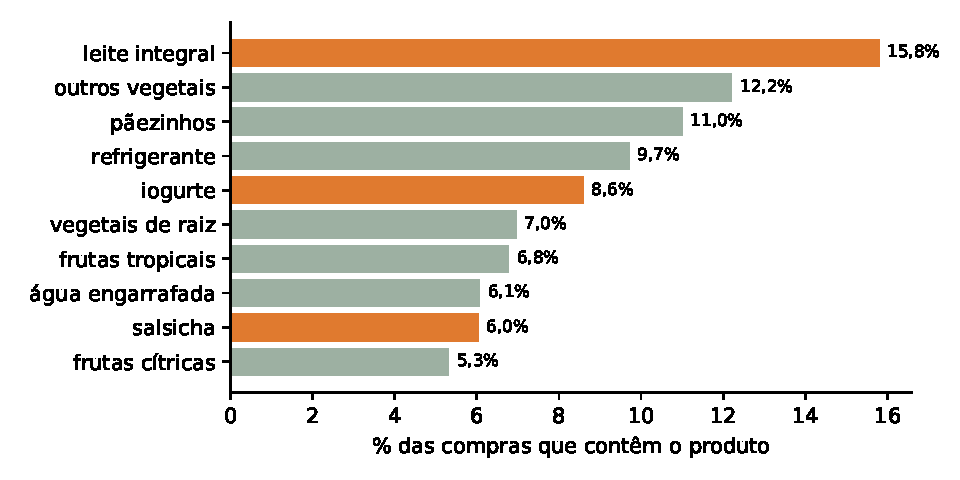
\includegraphics[width=0.85\textwidth]{figuras/itens_frequentes.pdf}
\caption{Os dez produtos mais frequentes. Em laranja, os produtos removidos na segunda rodada (a salsicha alemã, fora desta lista, também foi removida).}
\label{fig:itens}
\end{figure}

% ---------------------------------------------------------------
\section{Metodologia}

A análise foi implementada em Python com as bibliotecas \texttt{pandas} e \texttt{mlxtend}~\cite{raschka2018}, em cinco etapas:

\begin{enumerate}
  \item leitura do CSV;
  \item agrupamento dos registros por cliente e data, formando as transações (mantidas as que têm dois ou mais itens);
  \item codificação \emph{one-hot} com \texttt{TransactionEncoder}, que gera uma coluna verdadeiro/falso por produto;
  \item busca dos conjuntos frequentes com \texttt{apriori};
  \item geração das regras com \texttt{association\_rules}, ordenadas por lift e confiança.
\end{enumerate}

Foram feitas duas rodadas, com os parâmetros da Tabela~\ref{tab:parametros}. Na segunda, os itens que dominavam as regras da primeira (leite integral, iogurte, salsicha e salsicha alemã) foram removidos da base antes da mineração, e o suporte mínimo foi reduzido para captar relações entre produtos menos frequentes.

\begin{table}[H]
\centering
\caption{Parâmetros das duas rodadas.}
\label{tab:parametros}
\begin{tabular}{lrr}
\toprule
 & Rodada 1 & Rodada 2 \\
\midrule
Itens removidos & nenhum & 4 dominantes \\
Transações analisadas & \NumComprasRUm & \NumComprasRDois \\
Suporte mínimo & 0,1\% & 0,05\% \\
Equivale a (transações) & \MinComprasRUm & \MinComprasRDois \\
Lift mínimo & 1,0 & 1,1 \\
Conjuntos frequentes & \NumFrequentesRUm & \NumFrequentesRDois \\
Regras geradas & \NumRegrasRUm & \NumRegrasRDois \\
Regras distintas (sem espelhos) & \NumRegrasUnicasRUm & \NumRegrasUnicasRDois \\
\bottomrule
\end{tabular}
\end{table}

\paragraph{Pares espelhados.} Como $A \rightarrow B$ e $B \rightarrow A$ têm o mesmo lift, cada par aparece duas vezes na saída. Nas tabelas deste relatório, mantivemos apenas o sentido de maior confiança.

\paragraph{Teste de significância.} Para cada regra, foi aplicado o teste exato de Fisher (unilateral) à tabela $2\times 2$ que cruza a presença de $A$ com a presença de $B$. A hipótese nula é de independência entre antecedente e consequente. Como muitas regras são testadas ao mesmo tempo, também foram aplicadas a correção de Bonferroni e o controle da taxa de falsas descobertas de Benjamini--Hochberg~\cite{benjamini1995}.

% ---------------------------------------------------------------
\section{Resultados}

\subsection{Primeira rodada}

A Tabela~\ref{tab:rodada1} lista as dez regras distintas de maior lift. O topo é ocupado pelo trio iogurte, leite integral e salsicha, que aparece em três das quatro primeiras regras.

\begin{table}[H]
\centering
\caption{Rodada 1: as dez regras distintas de maior lift (suporte mínimo de 0,1\%). ``Compras'' é o número de transações que contêm a regra completa; $p$ é o p-valor do teste exato de Fisher, sem correção.}
\label{tab:rodada1}
\small
\begin{tabularx}{\textwidth}{XrRRrr}
\toprule
Regra & Compras & Suporte\newline(\%) & Confiança\newline(\%) & Lift & $p$ \\
\midrule
iogurte, leite integral $\rightarrow$ salsicha & 22 & 0,15 & 13,2 & 2,18 & 0,0005 \\
leite integral, salsicha $\rightarrow$ iogurte & 22 & 0,15 & 16,4 & 1,91 & 0,0023 \\
chocolate especial $\rightarrow$ frutas cítricas & 21 & 0,14 & 8,8 & 1,65 & 0,016 \\
iogurte, salsicha $\rightarrow$ leite integral & 22 & 0,15 & 25,6 & 1,62 & 0,013 \\
farinha $\rightarrow$ frutas tropicais & 16 & 0,11 & 11,0 & 1,62 & 0,039 \\
bebidas $\rightarrow$ salsicha & 23 & 0,15 & 9,3 & 1,54 & 0,027 \\
leite integral, refrigerante $\rightarrow$ salsicha & 16 & 0,11 & 9,2 & 1,52 & 0,061 \\
guardanapos $\rightarrow$ folhados/doces & 26 & 0,17 & 7,9 & 1,52 & 0,023 \\
queijo processado $\rightarrow$ vegetais de raiz & 16 & 0,11 & 10,5 & 1,51 & 0,064 \\
queijo duro $\rightarrow$ maçã/pera & 16 & 0,11 & 7,3 & 1,48 & 0,075 \\
\bottomrule
\end{tabularx}

\end{table}

A regra mais forte, \emph{iogurte + leite integral $\rightarrow$ salsicha}, tem lift de \MelhorLift: quem leva iogurte e leite tem 2,2 vezes mais chance de levar salsicha do que um cliente qualquer. Ainda assim, apenas \MelhorConf\% desses clientes levam salsicha, e o trio aparece em \MelhorCompras{} das \NumComprasRUm{} transações. A confiança máxima entre todas as regras da rodada é de \MaxConfRUm\%.

\begin{figure}[H]
\centering
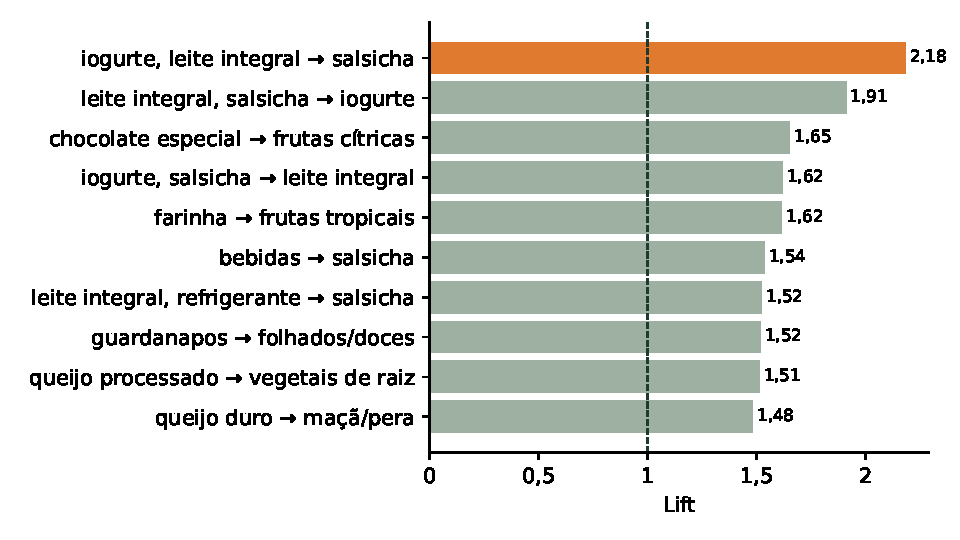
\includegraphics[width=0.9\textwidth]{figuras/lift_rodada1.pdf}
\caption{Lift das dez regras da Tabela~\ref{tab:rodada1}. A linha tracejada marca lift igual a 1 (independência).}
\label{fig:lift}
\end{figure}

A Figura~\ref{fig:dispersao} mostra todas as \NumRegrasRUm{} regras da rodada. \PctSupBaixo\% delas têm suporte abaixo de 0,2\%, e \PctConfVinte\% têm confiança abaixo de 20\%. Lift e confiança têm correlação fraca (\CorrLiftConf): as regras de maior lift não são, em geral, as de maior confiança.

\begin{figure}[H]
\centering
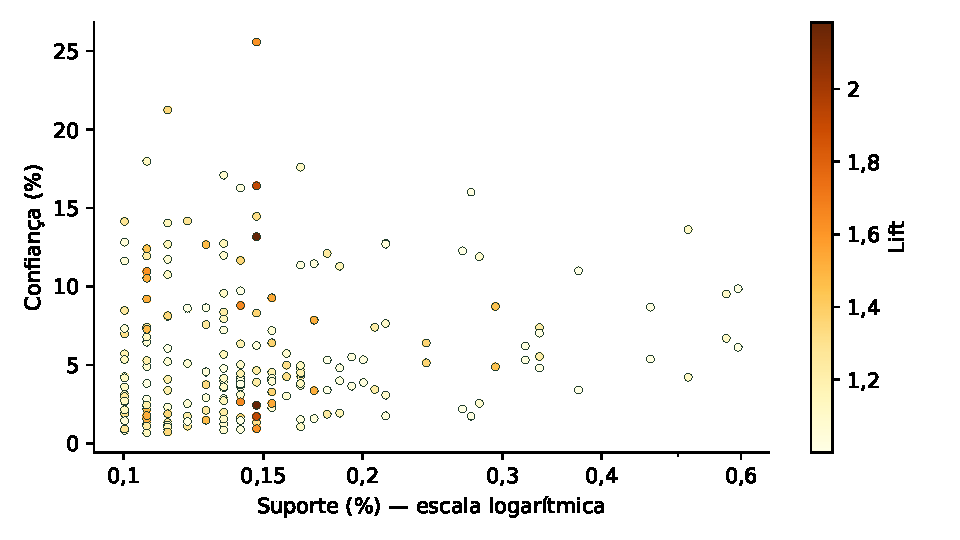
\includegraphics[width=0.9\textwidth]{figuras/dispersao_rodada1.pdf}
\caption{Suporte e confiança de todas as regras da rodada 1, coloridas pelo lift.}
\label{fig:dispersao}
\end{figure}

\subsection{Segunda rodada: sem os itens dominantes}

Sem os itens dominantes, aparecem associações que fazem sentido na cozinha, como presunto e conservas, ervas e óleo, e macarrão e carne moída (Tabela~\ref{tab:rodada2}). Os lifts são maiores que na primeira rodada, mas cada regra se apoia em apenas 7 a 11 transações.

\begin{table}[H]
\centering
\caption{Rodada 2: as dez regras distintas de maior lift, sem os itens dominantes (suporte mínimo de 0,05\%).}
\label{tab:rodada2}
\small
\begin{tabularx}{\textwidth}{XrRRrr}
\toprule
Regra & Compras & Suporte\newline(\%) & Confiança\newline(\%) & Lift & $p$ \\
\midrule
conservas $\rightarrow$ presunto & 8 & 0,07 & 6,3 & 3,32 & 0,0029 \\
ervas $\rightarrow$ óleo & 7 & 0,06 & 4,7 & 2,76 & 0,014 \\
macarrão $\rightarrow$ carne moída & 7 & 0,06 & 6,4 & 2,67 & 0,016 \\
carne de porco, frutas cítricas $\rightarrow$ outros vegetais & 7 & 0,06 & 35,0 & 2,60 & 0,012 \\
queijo macio $\rightarrow$ carne moída & 9 & 0,07 & 6,2 & 2,56 & 0,0087 \\
frutas cítricas, outros vegetais $\rightarrow$ carne de porco & 7 & 0,06 & 9,7 & 2,34 & 0,030 \\
adoçante $\rightarrow$ refrigerante & 7 & 0,06 & 25,0 & 2,27 & 0,029 \\
vinho tinto/rosé $\rightarrow$ salgadinho & 7 & 0,06 & 4,8 & 2,20 & 0,040 \\
pastas doces $\rightarrow$ maçã/pera & 8 & 0,07 & 11,8 & 2,14 & 0,032 \\
pastas doces $\rightarrow$ frutas tropicais & 11 & 0,09 & 16,2 & 2,12 & 0,013 \\
\bottomrule
\end{tabularx}

\end{table}

\subsection{Significância estatística}

Isoladamente, \SigRUm{} das dez regras da primeira rodada e \SigRDois{} das dez da segunda têm $p < 0{,}05$. Porém, as regras do topo foram escolhidas entre \NumRegrasUnicasRUm{} e \NumRegrasUnicasRDois{} candidatas, o que aumenta a chance de encontrar associações por acaso.

Com a correção de Bonferroni, o limite passa a ser de \AlfaBonfRUm{} na primeira rodada e \AlfaBonfRDois{} na segunda. O menor p-valor da primeira rodada, o da regra principal, é \MenorPRUm{}, ligeiramente acima do limite; na segunda rodada, o menor é \MenorPRDois. Assim, nenhuma regra se mantém significativa. O critério de Benjamini--Hochberg, menos conservador, leva à mesma conclusão: o menor valor $q$ é \MenorQRUm{} na primeira rodada e \MenorQRDois{} na segunda, ambos acima de 0,05.

% ---------------------------------------------------------------
\section{Discussão}

As regras encontradas são coerentes com hábitos de compra conhecidos. O trio iogurte, leite e salsicha sugere compras de rotina, ligadas a café da manhã e lanches. Os pares da segunda rodada lembram ingredientes de uma mesma receita: macarrão com carne moída, ervas com óleo, presunto com conservas.

Se confirmadas, essas regras poderiam orientar ações como:
\begin{itemize}
  \item \textbf{layout da loja:} aproximar macarrão e carne moída, ou ervas e óleo;
  \item \textbf{combos:} um ``kit café da manhã'' com iogurte, leite e salsicha;
  \item \textbf{recomendação:} sugerir conservas a quem coloca presunto no carrinho on-line.
\end{itemize}
Como as evidências são fracas, cada ação deveria ser testada antes, por exemplo com um experimento A/B que compare vendas com e sem a mudança.

% ---------------------------------------------------------------
\section{Limitações}

\begin{itemize}
  \item \textbf{Suporte baixo.} O suporte mínimo de 0,1\% equivale a cerca de \MinComprasRUm{} transações, e o de 0,05\% a cerca de \MinComprasRDois. Regras com tão poucos casos podem ser coincidência, como mostrou a análise de significância.
  \item \textbf{Confiança baixa.} Mesmo nas melhores regras, a maior parte de quem leva o antecedente não leva o consequente.
  \item \textbf{Transações pequenas.} Com média de \MediaItens{} itens, cada compra tem poucas combinações possíveis. Agrupar por cliente e data pode também juntar ou separar compras de forma imprecisa.
  \item \textbf{Bases diferentes entre rodadas.} Remover itens descarta transações (restaram \NumComprasRDois), então os suportes das duas rodadas não são comparáveis.
  \item \textbf{Escolha dos itens removidos.} Leite integral, iogurte e salsicha estão entre os dez mais frequentes, mas outros vegetais, pãezinhos e refrigerante, ainda mais frequentes que o iogurte e a salsicha, foram mantidos. A escolha seguiu as regras do topo, e não um critério de frequência, que seria mais objetivo.
\end{itemize}

% ---------------------------------------------------------------
\section{Conclusão}

O Apriori encontrou \NumFrequentesRUm{} conjuntos frequentes em \NumCompras{} compras e revelou associações plausíveis: o trio iogurte, leite integral e salsicha, com lift de \MelhorLift, e, sem os itens dominantes, pares de ingredientes de receitas. A análise estatística, porém, mostra que nenhuma regra resiste à correção para comparações múltiplas. Os resultados devem ser lidos como tendências a investigar, não como padrões confirmados.

Como trabalhos futuros, sugerimos: usar uma base maior ou um período mais longo; escolher os itens a remover por critério de frequência; comparar o Apriori com o FP-Growth; e validar as regras mais promissoras com experimentos na loja.

% ---------------------------------------------------------------
\begin{thebibliography}{9}

\bibitem{agrawal1993}
AGRAWAL, R.; IMIELIŃSKI, T.; SWAMI, A. Mining association rules between sets of items in large databases. In: \emph{Proceedings of the ACM SIGMOD International Conference on Management of Data}. 1993. p.~207--216.

\bibitem{agrawal1994}
AGRAWAL, R.; SRIKANT, R. Fast algorithms for mining association rules. In: \emph{Proceedings of the 20th International Conference on Very Large Data Bases (VLDB)}. 1994. p.~487--499.

\bibitem{brin1997}
BRIN, S.; MOTWANI, R.; ULLMAN, J. D.; TSUR, S. Dynamic itemset counting and implication rules for market basket data. In: \emph{Proceedings of the ACM SIGMOD International Conference on Management of Data}. 1997. p.~255--264.

\bibitem{benjamini1995}
BENJAMINI, Y.; HOCHBERG, Y. Controlling the false discovery rate: a practical and powerful approach to multiple testing. \emph{Journal of the Royal Statistical Society: Series B}, v.~57, n.~1, p.~289--300, 1995.

\bibitem{raschka2018}
RASCHKA, S. MLxtend: providing machine learning and data science utilities and extensions to Python's scientific computing stack. \emph{Journal of Open Source Software}, v.~3, n.~24, p.~638, 2018.

\bibitem{groceries}
DEDHIA, H. \emph{Groceries dataset}. Kaggle, 2020. Disponível em: \url{https://www.kaggle.com/datasets/heeraldedhia/groceries-dataset}.

\end{thebibliography}

\end{document}
